% path for images
\graphicspath{{assets/motivation/}}

\section[Motivation]{Motivation}

%%
\begin{frame}{Why going Quantum ?}
	Until now, we’ve relied on supercomputers to solve most problems. These are very large classical computers, often with thousands of classical CPU and GPU cores. However, supercomputers are not very good at solving certain types of problems, which seem easy at first glance. 
	
	\begin{center}
	    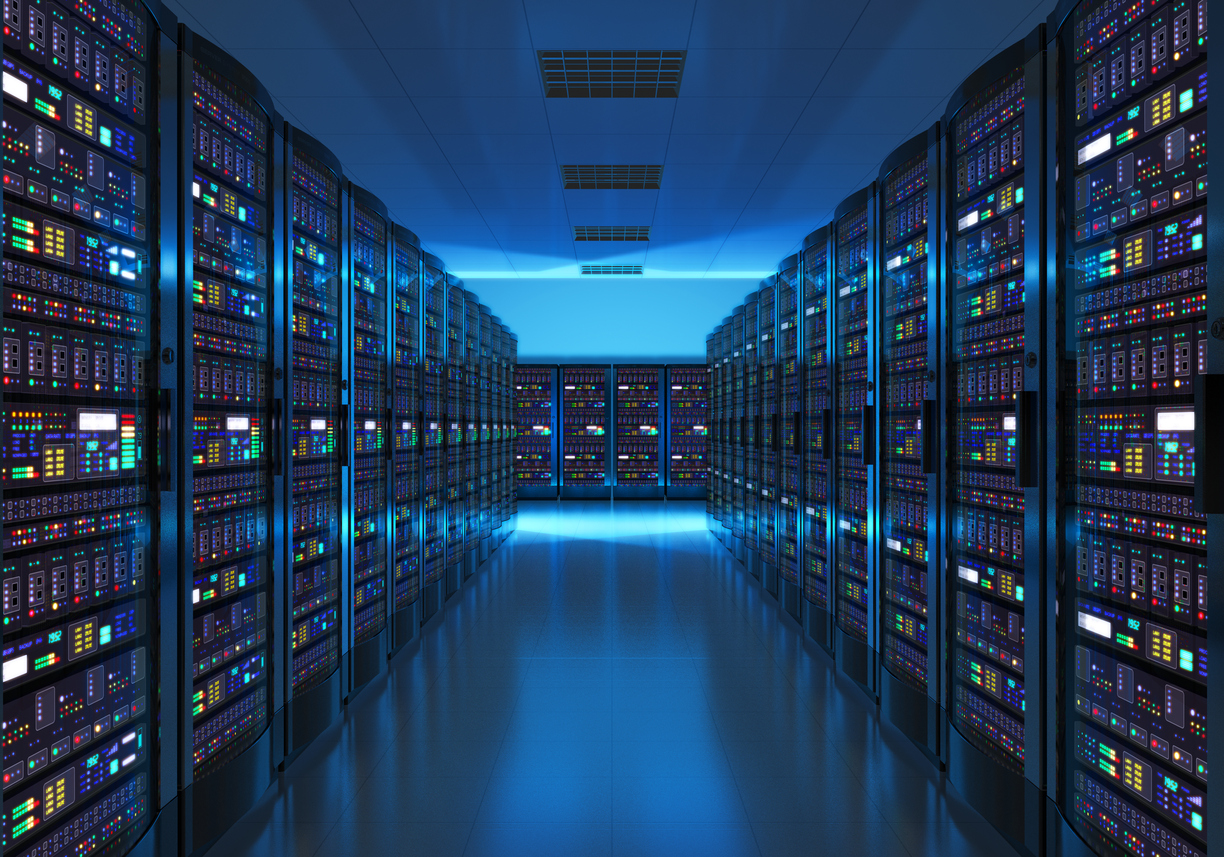
\includegraphics[width=.75\linewidth, height=.55\textheight]{server-room}
	\end{center}
\end{frame}

%%
\begin{frame}{Why going Quantum ? A simple example}
	
Imagine you want to seat 10 fussy people at a dinner party, where there is only one optimal seating plan out of all the different possible combinations. How many different combinations would you have to explore to find the optimal?

Can you guess how many \alert{combinations}\footnote{Example from IBM's website \url{https://www.ibm.com/quantum-computing/what-is-quantum-computing/}} ?
\end{frame}


%% animation
\begin{frame}[<+- | only+>]{Why going Quantum ? A simple example}
	\metroset{block=fill}
	
	
	\begin{exampleblock}{For 2 people}
		2 Total combinations.
	\end{exampleblock}

	\begin{block}{For 5 people}
		120 Total combinations.
	\end{block}
	

	\begin{alertblock}{For 10 people}
		Over 3 Million of total combinations!!!
	\end{alertblock}	
	
	\begin{itemize}
		\item Supercomputers don't have the working \alert{memory} to hold the myriad combinations of real world problems.
		\item Supercomputers have to analyze each combination one after another, which can take a long \alert{time}.
	\end{itemize}
\end{frame}

\begin{frame}{Why going Quantum?}
\begin{figure}[H]
    \centering
    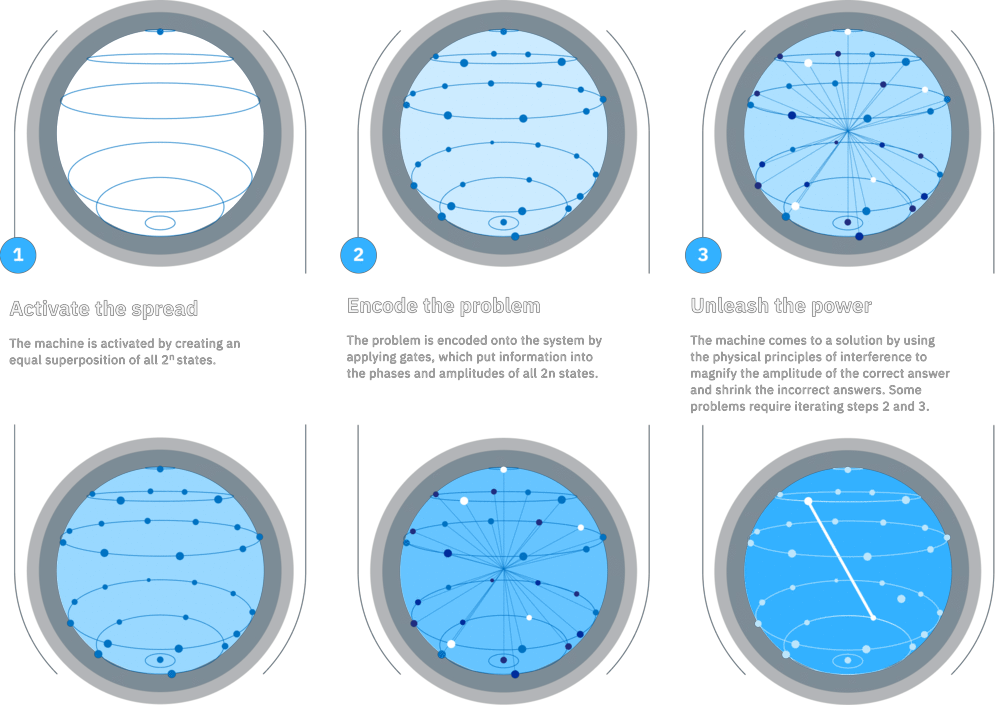
\includegraphics[width=.7\linewidth]{ quantumsup.png}
    %\caption{Quantum Supremacy}
\end{figure}
\begin{itemize}
    \item Quantum computers can create vast multidimensional spaces in which to represent these very large problems. Classical supercomputers cannot do this.
   
\end{itemize}
  
\end{frame}

\begin{frame}{Why going Quantum ?}
\begin{itemize}
 \item Referring to the "10 fussy people at a dinner party" problem, with \alert{22 qubit} we can represent $2^{22} = 4194304$ states.
    \item The computation may be carried out on all those numbers in a \alert{single parallel computation}. This built-in parallelism is the key to the power of quantum computers.
\end{itemize}
    
\end{frame}


%%
\begin{frame}{How is a Quantum computer programmed?}
\begin{figure}[H]
    \centering
    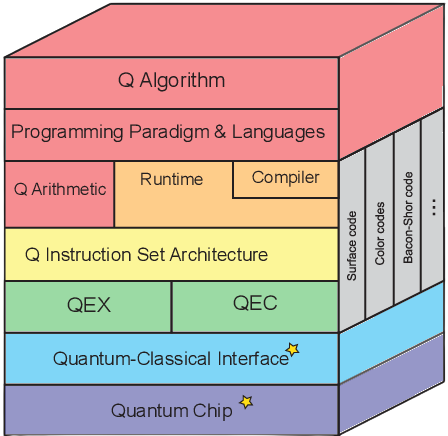
\includegraphics[width=.4\linewidth]{ Hto8a.png}
    %\caption{Quantum Computer Architecture}
\end{figure}
There is an \alert{interface} between quantum mechanical processes and classical computer processes. Through this interface, input data from a a classical computing device can be fed into a quantum circuit.
\end{frame}

%%
\begin{frame}{How is a Quantum computer programmed?}
    \begin{itemize}
        \item \alert{Quantum Circuits} are constructed from Quantum Registers.
        \item \alert{Quantum Register} is a type of circuit construction from logical qubits. 
        \item \alert{Logical Qubits} can create different permutations and combinations of physical qubit manifestations.
    \end{itemize}
\end{frame}

%%
\begin{frame}[fragile]{What are Quantum Computers good at ?}
    \begin{figure}[h!]
         \captionsetup[subfloat]{labelformat=empty}
         \subfloat[Linear Algebra]{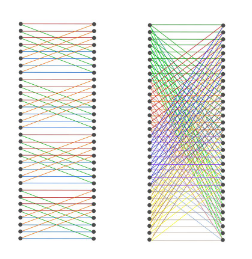
\includegraphics[width=0.3\linewidth]{linalg}} \quad
		 \subfloat[Sampling]{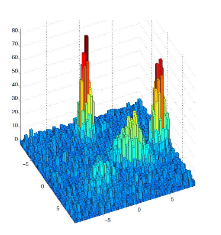
\includegraphics[width=0.3\linewidth]{sampling}} \quad
		 \subfloat[Optimization]{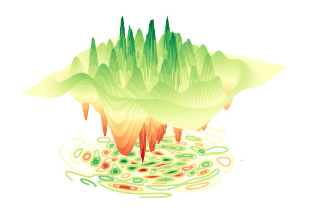
\includegraphics[width=0.33\linewidth, height=0.38\textheight]{optimiz}} 
    \end{figure}
\end{frame}


%%
\begin{frame}[fragile]{A Growing Interest in the field}
	\begin{itemize}
	 \item Many frameworks from big techs (IBM's Qiskit, PennyLane, Google's TensorFlow Quantum, Microsoft Q\#, ...)
	 \item  A significant growth in research
	   \begin{figure}[!htb]
	           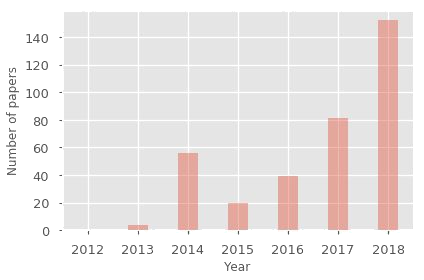
\includegraphics[width=0.5\linewidth]{plot_interest}\quad
	    \end{figure}
	 \item  All the Big Techs (Microsoft, Google, IBM, Nvidia ... ) have/want a quantum computer
	 \item  Growing interest in the field of Quantum Programming Languages
	\end{itemize}
\end{frame}